%Vor dem Editieren die Styleguide auf dem Server lesen!
%Include Header
%Angaben zum Dokument
\newcommand*\myauthor{KKK K\"oppel, K\"oppel und Konsortium}
\newcommand*\mytitle{Digitaltechnik 2 Zusammenfassung}
\newcommand*\mydate{\today}

%Schriftgroesse, Layout, Papierformat, Gleichungen Linksbuendig
\documentclass[10pt,twoside,a4paper,fleqn]{article}

%Abmessungen Layout
\usepackage[left=1cm,right=1cm,top=1cm,bottom=1cm,includeheadfoot]{geometry}

%Package fuer Umlaute
\usepackage[latin1]{inputenc}
\usepackage[T1]{fontenc}
\usepackage[latin1]{inputenc}

%Package fuer Deutsch
\usepackage[ngerman]{babel}

%Formeln
\usepackage{amsmath}
%Spezielle Symbole in Formeln
\usepackage{amssymb}
%Sonderzeichen
\usepackage{textcomp}
%Bilder und Grafiken
\usepackage{graphicx}
%Textfarben
\usepackage{color}
%Fliesstext
\usepackage{wrapfig}
%Header und Footer
\usepackage{fancyhdr}
%Teile des Dokuments Mehrspaltig
\usepackage{multicol}
%Rotieren von Elementen (Bilder, Tabellen...)
\usepackage{rotating}
%Schriftart
\usepackage[scaled]{helvet}
\renewcommand*\familydefault{\sfdefault}
%Package f�r Code
\usepackage{listings}
%Seitenaufbau
\pagestyle{fancy} %eigener Seitenstil
%\fancyhf{}

%Linker Header
\lhead{\mytitle}


%Rechter Header
\rhead{\leftmark}
%Linker Footer
\lfoot{\myauthor}
%Center Footer
\cfoot{\thepage}
%Rechter Footer
\rfoot{\mydate}
%Text Linksbuendig, unregelmaessiger rechter Rand
\raggedright


%Document Anfang
\begin{document}

%Input von Kapiteln anschliessend
%\input{sections/kapitelname}
%Input von Kapiteln auf neuer Seite
%\include{sections/kapitelname}
\part*{\mytitle}
\section{Testbench}
\subsection{Eigenschaften}
\begin{itemize}
  \setlength{\itemsep}{1pt}
  \setlength{\parskip}{0pt}
  \setlength{\parsep}{0pt}
  \item Zu pr�fende Komponente wird unver�ndert aus Bibliothek �bernommen.
  (Component).
  \item Testbench muss verschiedene Architekturen einfach einbinden k�nnen.
  \item Innerhalb der Architektur der Testbench d�rfen auch nicht
  synthetisierbare VHDL Konstrukte verwendet werden. (z.B.: for-Schleife)
  \item Simulationszeit = Reale Zeit $\neq$ Rechenzeit der Simulation.
  \item Normalerweise 3 Prozesse (clock, stimuli, response).
\end{itemize}
\newpage
\subsection{Codebeispiel}
  \lstinputlisting[language=VHDL,tabsize=2]{code/testbench.vhdl}
\newpage  
\subsection{Timing Simulation}
\begin{multicols}{2}
  \subsubsection{Delta Time}
    Wird Verz�gerungszeit einer Operation nicht explizit angegeben, so wird mit
    $ \Delta $ time gerechnet (meistens 0).
  \subsubsection{Inertial}
    Signalzuweisung mit after:\\
    \lstinputlisting[language=VHDL,tabsize=2]{code/inertial_delay.vhdl}
    Y �ndert Wert nur, wenn \"Anderung des Eingangs l�nger wirksam ist als
    delay ist. Spikes werden nicht ber�cksichtigt.
  \subsubsection{Transport}
    Ausgang wird in jedem Fall um delay gegen�ber Eingang verschoben.
    \lstinputlisting[language=VHDL,tabsize=2]{code/transport_delay.vhdl}
\end{multicols}
\section{Key Concepts}
\begin{tabular}{ll}
  Key Concept I: & Schaltungshierarchie und Verbindung von Sub-Bl�cken (hierarchy and connectivity).\\
  Key Concept II: & Nebenl�ufige (concurrent) Prozesse und Prozess-Interaktion.\\
  Key Concept III: & Modellierung des elektrischen Verhaltens von Signalen.\\
  Key Concept IV: & Event-Based time: Simulationsmodell, das auf Events und nicht auf kontinuierlicher Zeit beruht.\\
  Key Concept V: & Parametrisierung von Modellen.\\
\end{tabular}
\section{Sequentielle Systeme}
\subsection{Kombinatorische und sequentielle Systeme}
	\begin{tabular}{|p{9cm}|p{9cm}|}
		\hline
		\textbf{Kombinatorische Systeme} & \textbf{Sequentielle Systeme} \\
		\hline
		Zustandsfrei & Zustandsbehaftet \\
		\hline
		Ausg"ange sind funktional von den Eing"angen abh"angig &
		Vergangenes Verhalten und Eing"ange bestimmen momentanen Zustand und Ausg"ange\\
		\hline
	\end{tabular}

\subsection{Eigenschaften Sequenzieller systeme}
	\begin{multicols}{2}
		\begin{itemize}
			\setlength{\itemsep}{1pt}
			\setlength{\parskip}{0pt}
			\setlength{\parsep}{0pt}
			  
		  \item Ausg"ange sind von Eing"angen \textbf{und} Zustand des Systems bestimmt
		  \item Grundelemnte f�r Ged"achtnis: FlipFlop
		  \item Seq. Systeme k�nnen mit Zustandsdiagrammen dargestellt werden
		  \item Wechsel des Zustandes zun Zeitpunkt einer Flanke des Taktsignals
		  \item Zustandwechsel jederzeit
		\end{itemize}
	\end{multicols}


\subsection{Dastellung sequentieller Systeme}
	\begin{multicols}{4}
		\subsubsection{Statediagramm}
			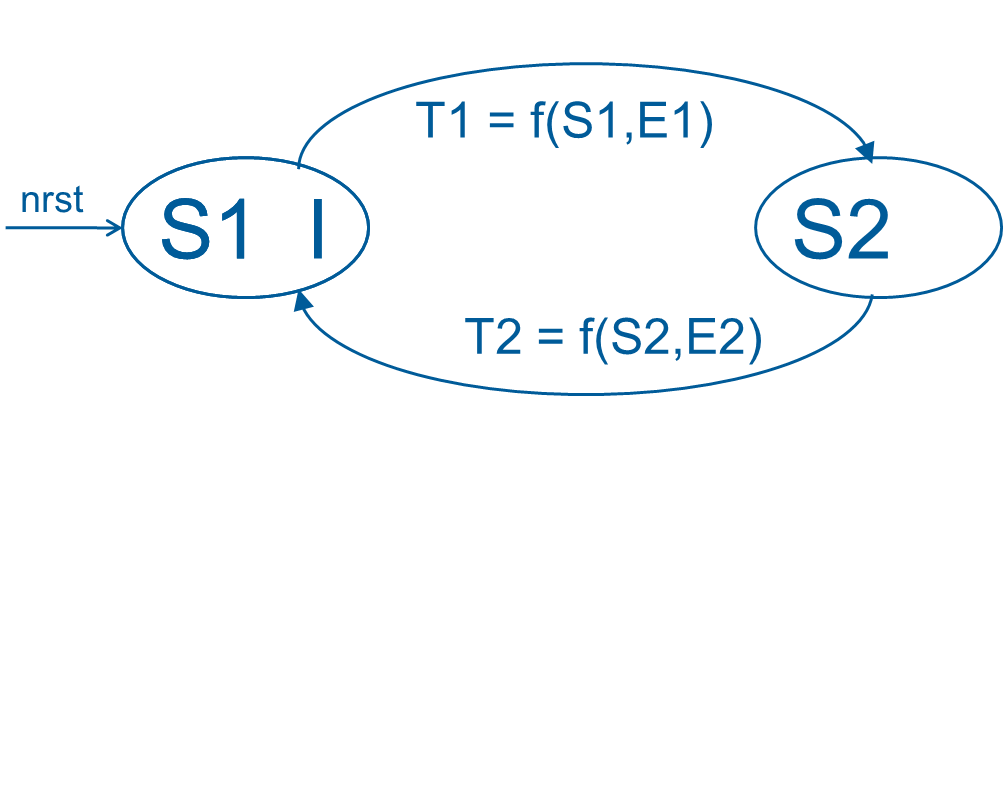
\includegraphics[width=0.25\textwidth]{pics/seq_uml}\\
			\begin{itemize}
			  \setlength{\itemsep}{1pt}
			  \setlength{\parskip}{0pt}
			  \setlength{\parsep}{0pt}
			  
			  \item S: Menge der Zust"ande mit Zustandsaktionen
			  \item $I\subseteq S:$ Initalzust"ande
			  \item T: "Ubergangsrelation $f(S,E)$
			  \item E: Eing"ange
			\end{itemize}
			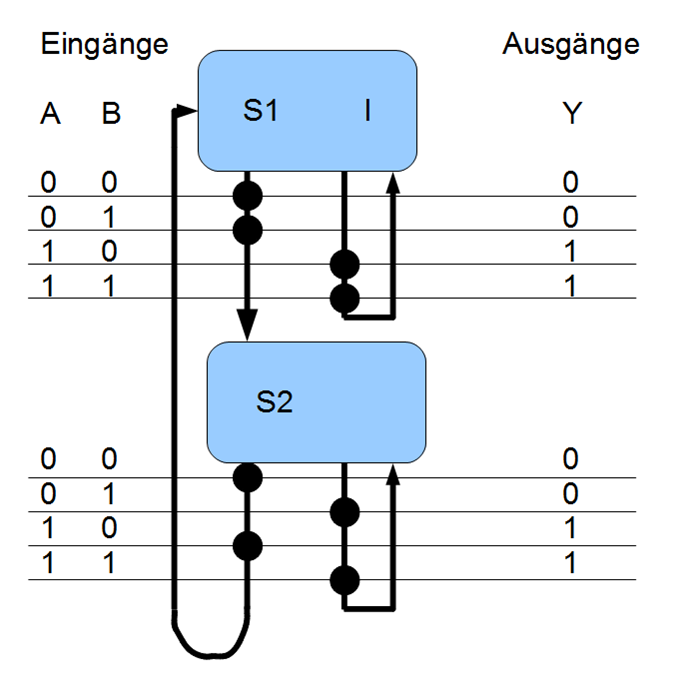
\includegraphics[width=0.25\textwidth]{pics/seq_statediagramm}\\
			\textbf{Vorgehen}
			\begin{enumerate}
			  \setlength{\itemsep}{1pt}
			  \setlength{\parskip}{0pt}
			  \setlength{\parsep}{0pt}
			
			  \item Zust"ande zeichnen und Benennen
			  \item Initalzustand bestimmen
			  \item Eing"ange systematisch auflisten
			  \item Zustands "uberg"ange (Transitionen) bestimmen
			  \item Ausg"ange einzeichnen
			\end{enumerate}
	\end{multicols}
	\subsubsection{Zustandstabelle}
	\begin{multicols}{3}
			\textbf{Vorgehen}
			\begin{enumerate}
			  \setlength{\itemsep}{1pt}
			  \setlength{\parskip}{0pt}
			  \setlength{\parsep}{0pt}
			
			  \item Ausgangspunkt = Warheitstabelle\\
			  \item Wird pro Zustand aufgeschieben\\
			  \item Erg"anzt mit Folgezustand\\
			\end{enumerate}
		
			\begin{tabular}{|l|l|l|}
				\multicolumn{3}{c}{\textbf{Eingangsvariable}}\\
				\hline
				$In_1$ & $In_2$ & $\cdots$ \\
				\hline
				0 & 0 & $\cdots$ \\
				\hline
				0 & d & $\cdots$ \\
				\hline
				$\cdots$ & $\cdots$ & $\cdots$ \\
				\hline
			\end{tabular}
			
			\begin{tabular}{|l|l|l|}	
				\multicolumn{3}{c}{\textbf{Ausgangsvariable}}\\
				\hline
				$In_1$ & $In_2$ & $\cdots$ \\
				\hline
				0 & 0 & $\cdots$ \\
				\hline
				0 & d & $\cdots$ \\
				\hline
				$\cdots$ & $\cdots$ & $\cdots$ \\
				\hline
			\end{tabular}
	\end{multicols}			

\subsection{Zustandcodes}
	\begin{multicols}{2}
	\begin{itemize}
		\setlength{\itemsep}{1pt}
		\setlength{\parskip}{0pt}
		\setlength{\parsep}{0pt}
			
		\item Zust�nde werden der Reihe nach bin�r durch nummeriert.
		\item Ben�tigte Anzahl Speicherstellen $k$ f�r eine Anzahl Zust�nder $p$:\\
		$p\leq 2^k$ | $k=\log_2(p)=\frac{\log_{10}(p)}{\log_{10}(2)}$
		\item Anzahl M�glicher Speicherstellen:\\
		$q=\frac{(2^k)!}{(2^k-p)!}$
		\item \textbf{Alternative:} Graycode, es wechselt nur 1 Bit\\
	\end{itemize}
	\end{multicols}
	
\subsubsection{ONE-HOT Zustandscodierung}
	Pro Code wird genau eine Speicherstelle TURE. Alle anderen werden FALSE.
\subsubsection{ONE-COLD Zustandscodierung}
	Pro Code wird genau eine Speicherstelle FALSE. Alle anderen werden TURE.
	
\subsection{Sequentielle Systeme in VHDL}
\lstinputlisting[language=VHDL,tabsize=2]{code/sequentiell.vhdl}


\section{Endliche Zustandsautomaten, Finite State Machine}
\subsection{Grundlegende Eigenschaften}
Eine FMS ist ein Geschlossenes Modell mit einer endlichen Anzahl von Zust�nden,
Zustands�berg�ngen und Aktionen.\\
\textbf{Sinn:} Mathematische Abstraktion, Grundlage theoretischer
Betrachtungen, Ausgangspunkt systematischer parktischer Realisierung.\\
\textbf{Anweundungen:} Informatik (Parser, Compiler, Game)\\
Technik, digitale Schaltungen (Kaffee-Automat, Parkticket, \ldots)\\
Kommunikationstechnik (Protokolldesign)\\
  \subsubsection{Grundstruktur}
  \begin{multicols}{3}
    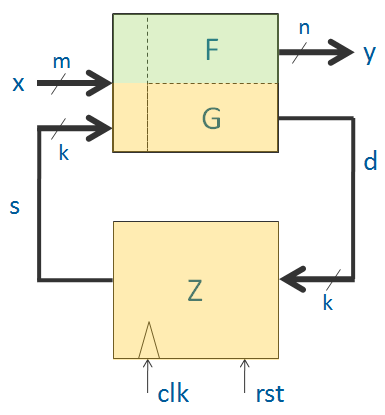
\includegraphics[width=0.2\textwidth]{pics/fsm_grundlage}
    \textbf{Kombinatorische Logik F/G}\\
    Generiert Ausg�nge\\ und Folgezustand.\\
    F = Funktion f�r Ausg�nge\\
    G = Funktion f�r Speicheransteuerung\\
    \textbf{Zustandsregister Z}\\
    Z = Zustansspeicher/register\\
    Sequentieller Teil des Systems,\\
    speichert aktuellen Zustand.\\
    \textbf{Signale}\\
    x = Eingangsvektor\\
    m = Anzahl Eing�nge\\
    y = Ausgangsvektor\\
    n = Anzahl Ausg�nge\\
    s = Zustandsvektor\\
    d = Folgezustand\\
    \textbf{Memory}\\
    k = Anzahl Speicherstellen\\
    
  \end{multicols}
  %Bild V4F7
\subsection{Mealy, Moore und Medwedjew}
\begin{tabular}{|p{6cm}|p{6cm}|p{6cm}|}
  \hline
  \textbf{Mealy-System} & \textbf{Moore-System} & \textbf{Medwedjew-System} \\
  \hline
  Grundsystem; komb. Logik F/G in zwei separate Bl�cke aufgeteilt & Wert der
  prim�ren Ausg�nge ist nur vom aktuellen Zustand des Systems abh�ngig. &
  Spezialfall des Moore-Systems: Prim�re Ausg�nge entsprechen dem Zustandsvektor \\
  \hline
  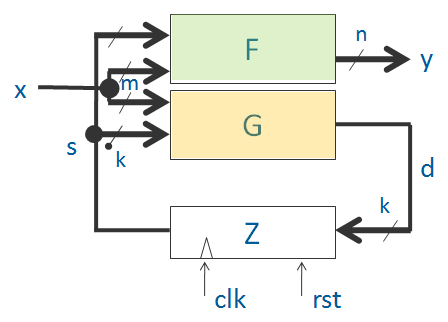
\includegraphics[width=0.3\textwidth]{pics/fsm_mealy} &
  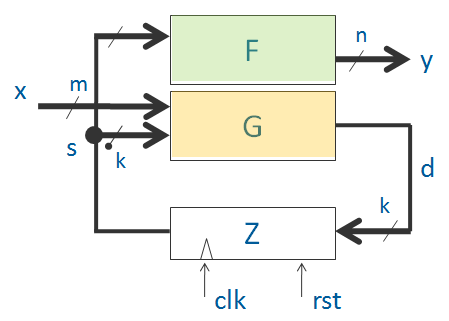
\includegraphics[width=0.3\textwidth]{pics/fsm_moore} &
  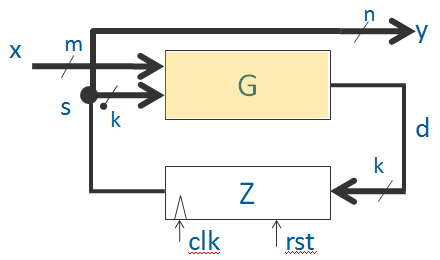
\includegraphics[width=0.3\textwidth]{pics/fsm_medwedjew} \\
  \hline
  Ausg�nge h�ngen vom momentanen Zustand und den aktuellen Eing�ngen ab.
  & Ausg�nge h�ngen nur vom momentanen Zustand ab und �ndern mit der
  Clock-Flanke & Die prim�ren Ausg�nge entsprechen dem Zustandsvektor.
  Ausgangsfunktion F degeneriert auf 1. \\
  \hline
  $ y[i] = F(x[i],x[i]) $ & $ y[i] = F(s[i]) $ & $ y[i] = s[i] := G(x[i-1],y[i-1]) $ \\
  $ d[i] = s[i+1] := G(x[i],s[i]) $ & $ d[i]=s[i+1] := G(x[i],s[i]) $ & $ 
  s[i+1]:=G(x[i],s[i])$ \\
  \hline
  Entwurf mit asynchronem Output. Ausgabe unabh�ngig vom Clock. & Allgemeiner Prototyp eines synchronen, sequentiellen Entwurfes. & Ausg�nge
  entsprechen den Zust�nden.\\
  \hline
  Lange Signalpfade! & Verz�gerung Latenzzeit & Zust�nde m�ssen gleich codiert
  werden wie Ausgangssignale\\
  \hline
  Mausefalle & & Die meisten Counter \\
  \hline
  %Code zu einzelnen Varianten hinzuf�gen V4 ab seite 21
\end{tabular}

\section{Parametrisierung}
VHDL kann Parameter an ein Modell �bergeben. Deklariert in
Schnittstellenbeschreibung. Dies macht den Code Flexibler und erlaubt die
wieder Verwendung von von Code\\

\subsection{Anwendung}
\begin{multicols}{2}
	\lstinputlisting[language=VHDL,tabsize=2]{code/parametrisierung.vhdl}
\end{multicols}

\subsection{Unterschiede der Konzepte}
\begin{tabular}{p{3cm}p{7.5cm}p{7.5cm}}
	Parameter fixiert zu \textbf{Desingetime} & VHDL Design mit Konstanten
	&Counter $0 \ldots 4$\\
	Parameter fixiert zu \textbf{Compiletime} & Gernic Konzept �bermittelt
	Information zu compiletime & Wiederverwendbarer Z�hler mit Z�hlerbereich 0
	$\ldots$ maxcount \\
	Parameter fixiert zur \textbf{Runtime} & Signale �bermitteln Informationen zur
	Runtime & Z�hlerbereich kann �ber Schalter eingestellt werden.
\end{tabular}
\section{Schiebeoperationen}
\subsection{Logische Schiebeoperatoren SLL, SRL}
	\begin{multicols}{2}
		\begin{itemize}
			\setlength{\itemsep}{1pt}
			\setlength{\parskip}{0pt}
			\setlength{\parsep}{0pt}
			
			\item Bits werden um eine Stelle geschoben.
			\item Freiwerdende Stelld wird mit Initalwert des des Basistyps aufgef�llt:
			=0.
			\item Aus dem Indexbereich hinausgeschobener Inhalt geht verloren.
		\end{itemize}
		\begin{center}
			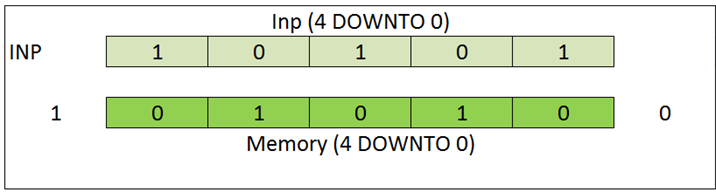
\includegraphics[width=.4\textwidth]{pics/logic_shift}
		\end{center}
	\end{multicols}
	
	\begin{multicols}{2}	
		\begin{lstlisting}[language=vhdl,tabsize=2]
			signal MEM: bit_vector (4 DOWNTO 0);
			MEM <= MEM sll 1;
		\end{lstlisting}
		
		\textbf{Anwendung:} Muliplikation / Divison mit $2^n$
	\end{multicols}
	
\subsection{Arithmetische Schiebeoperatoren SLA, SRA}
	\begin{multicols}{2}
		\begin{itemize}
			\setlength{\itemsep}{1pt}
			\setlength{\parskip}{0pt}
			\setlength{\parsep}{0pt}
			
			\item Bits werden um eine Stelle geschoben.
			\item Freiwerdende Stelle wird mit letztem geschobenem Bit aufgef�llt.
			\item Aus dem Indexbereich hinausgeschobener Inhalt geht verloren.
		\end{itemize}
		\begin{center}
			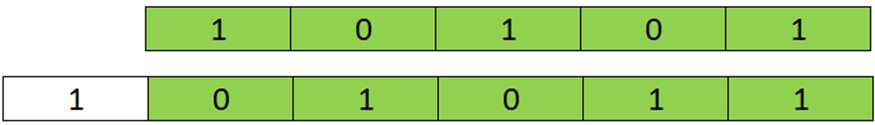
\includegraphics[width=.4\textwidth]{pics/arith_shift}
		\end{center}
	\end{multicols}
	
	\begin{multicols}{2}	
		\begin{lstlisting}[language=vhdl,tabsize=2]
			IMP <= sla 1;
		\end{lstlisting}
		
		\textbf{Anwendung:} Division mit $2^n$ bei sing-magnitude Darstellung (SRA).
	\end{multicols}

\subsection{Rotierende Schiebeoperatoren SLA, SRA}
	\begin{multicols}{2}
		\begin{itemize}
			\setlength{\itemsep}{1pt}
			\setlength{\parskip}{0pt}
			\setlength{\parsep}{0pt}
			
			\item Bits werden um eine Stelle geschoben.
			\item Freiwerdende Stelle wird mit vorderstem Bit der Kette aufgef�llt.
			\item Aus dem Indexbereich hinausgeschobener Inhalt wird hinten angeh�ngt.
		\end{itemize}
		\begin{center}
			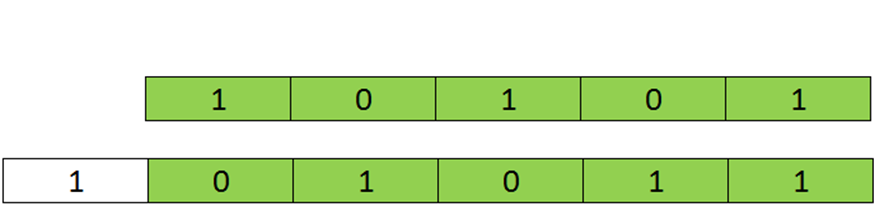
\includegraphics[width=.4\textwidth]{pics/rol_shift}
		\end{center}
	\end{multicols}
	
	\begin{multicols}{2}	
		\begin{lstlisting}[language=vhdl,tabsize=2]
			IMP <= rol 1;
		\end{lstlisting}
		
		\textbf{Anwendung:} Bitweise Analyse.
	\end{multicols}
		

\end{document}